\chapter{Lec TBL-2 - Moving Beyond Linearity}

\section{Introduction}
So far, we have mostly focused on linear models. Linear models are relatively simple to describe and implement, and have advantages over other approaches in terms of interpretation and inference. However, standard linear regression can have significant limitations in terms of predictive power.  In this chapter we relax the linearity assumption while still attempting to maintain as much interpretability as possible. We do this by examining very simple extensions of linear models like polynomial regression and step functions, as well as more sophisticated approaches such as splines and generalized additive models.

\begin{itemize}
    \item \textit{Polynomial regression} extends the linear model by adding extra predictors, obtained by raising each of the original predictors to a power. For example, a cubic regression uses three variables, $X, X^2$, and $X^3$, as predictors.

    \item \textit{Step functions} cut the range of a variable into $K$ distinct regions in order to produce a qualitative variable. This has the effect of fitting a piecewise constant function.

    \item \textit{Regression splines} are more flexible than polynomials and step functions, and in fact are an extension of the two. They involve dividing the range of $X$ into $K$ distinct regions. Within each region, a polynomial function is fit to the data. However, these polynomials are constrained so that they join smoothly at the region boundaries, or knots.

    \item \textit{Smoothing splines} are similar to regression splines, but arise in a slightly different situation. Smoothing splines result from minimizing a residual sum of squares criterion subject to a smoothness penalty.

    \item \textit{Generalized additive models} allow us to extend the methods above to deal with multiple predictors.

\end{itemize}

\section{Polynomial Regression}
Historically, the standard way to extend linear regression to settings in which the relationship between the predictors and the response is nonlinear has been to replace the standard linear model with a polynomial function
\begin{equation}
    y_i = \beta_0 + \beta_1x_i + \beta_2x_i^2 + ... + \beta_dx_i^d + \epsilon_i
    \label{polynomial-reg}
\end{equation}
This approach is known as \textit{polynomial regression}. The coefficients in \ref{polynomial-reg} can be easily estimated using least squares linear regression because this is just a standard linear model with predictors $x_i, x_i^2, ..., x_i^d$. Generally speaking, it is unusual to use $d$ greater than 3 or 4 because for large values of $d$, the polynomial curve can become overly flexible and can take on some very strange shapes.

\section{Step Functions}
Using polynomial functions of the features as predictors in a linear model imposes a global structure on the non-linear function of $X$. We can instead use step functions in order to avoid imposing such a global structure. Here we break the range of $X$ into \textit{bins}, and fit a different constant in each bin. This amounts to converting a continuous variable into an \textit{ordered categorical variable}.\\\\
In greater detail, we create cutpoints $c_1, c_2,...,c_K$ in the range of $X$, and then construct $K + 1$ new variables
\[
\begin{split}
    C_0(X) & = I(X<c_1),\\
    C_1(X) & = I(c_1 \leq X < c_2),\\
    C_2(X) & = I(c_2 \leq X < c_3),\\
    & .\\
    & .\\
    & .\\
    C_{K-1}(X) & = I(c_{K-1} \leq X < c_K),\\
    C_K(X) & = I(c_K \leq X)
\end{split}
\]
These are sometimes called \textit{dummy variables}. Notice that for any value of $X$, $C_0(X) + C_1(X) + ... + C_K(X) = 1$, since $X$ must be in exactly one of the $K + 1$ intervals. We then use least squares to fit a linear model using $C_1(X), C_2(X),...,C_K(X)$ as predictors.
\begin{equation}
    y_i = \beta_0 + \beta_1C_1(x_i) + \beta_2C_2(x_i) + ... + \beta_KC_K(x_i) + \epsilon_i
    \label{step-function}
\end{equation}
Note that when $X<c_1$, all of the predictors in \ref{step-function} are zero, so $\beta_0$ can be interpreted as the mean value of $Y$ for $X<c_1$. By comparison, $\beta_j$ represents the average increase in the response for $X$ in $c_j \leq X < c_{j+1}$ relative to $X<c_1$.
\\\\
Unfortunately, unless there are natural breakpoints in the predictors, piecewise-constant functions can miss the action.  Nevertheless, step function approaches are very popular in biostatistics and epidemiology, among other disciplines. For example, 5-year age groups are often used to define the bins.

\section{Basis Functions}
Polynomial and piecewise-constant regression models are in fact special cases of a \textit{basis function} approach. The idea is to have at hand a family of functions or transformations that can be applied to a variable $X$: $b_1(X), b_2(X), ..., b_K(X)$. Instead of fitting a linear model in $X$, we fit the model
\begin{equation}
    y_i = \beta_0 + \beta_1b_1(x_i) + \beta_2b_2(x_i) + ... + \beta_Kb_K(x_i) + \epsilon_i
    \label{basis}
\end{equation}
For polynomial regression, the basis functions are $b_j(x_i) = x_i^j$ and for piecewise constant functions they are $b_j(X_i) = I(c_j \leq x_i < c_{j+1})$. We can think of \ref{basis} as a standard linear model with predictors $b_1(X), b_2(X), ..., b_K(X)$. Hence, we can use least squares to estimate the unknown regression coefficients in \ref{basis}.  Importantly, this means that all of the inference tools for linear models are available in this setting.\\\\
Thus far we have considered the use of polynomial functions and piecewise constant functions for our basis functions; however, many alternatives are possible. For instance, we can use wavelets or Fourier series to construct basis functions. In the next section, we investigate a very common choice for a basis function: \textit{regression splines}.

\section{Regression Splines}
Now we discuss a flexible class of basis functions that extends upon the polynomial regression and piecewise constant regression approaches that we have just seen.

\subsection{Piecewise Polynomials}
Instead of fitting a high-degree polynomial over the entire range of $X$, \textit{piecewise polynomial regression} involves fitting separate low-degree polynomials over different regions of $X$. For example, a piecewise cubic polynomial works by fitting a cubic regression model of the form
\begin{equation}
     y_i = \beta_0 + \beta_1x_i + \beta_2x_i^2 + \beta_3x_i^3 + \epsilon_i
     \label{cubic-pol}
\end{equation}
where the coefficients $\beta_0, \beta_1, \beta_2$, and $\beta_3$ differ in different parts of the range of $X$. The points where the coefficients change are called \textit{knots}.A piecewise cubic polynomial with a single knot at a point $c$ takes the form
\[
y_i =
\begin{cases}
     \beta_{01} + \beta_{11}x_i + \beta_{21}x_i^2 + \beta_{31}x_i^3 + \epsilon_i & \text{if } x_i < c;\\
\beta_{02} + \beta_{12}x_i + \beta_{22}x_i^2 + \beta_{32}x_i^3 + \epsilon_i & \text{if } x_i \geq c.   
\end{cases}
\]
Each of these polynomial functions can be fit using least squares applied to simple functions of the original predictor (more details later). If we place $K$ different knots throughout the range of $X$, then we will end up fitting $K + 1$ different cubic polynomials. Note that we do not need to use a cubic polynomial. For example, we can instead fit piecewise linear functions. In fact, our piecewise constant functions defined previously are piecewise polynomials of degree 0. A piecewise cubic polynomial (4 parameters) fitted with a single knot uses a total of $4 \times 2 = 8$ \textit{degrees of freedom}. Basically, the degrees of freedom are the number of parameters to be estimated.

\subsection{Constraints and Splines}
The top left panel of the Figure below shows a piecewise cubic polynomial fit to
a subset of the Wage data, with a single knot at $age=50$. 
\begin{center}
    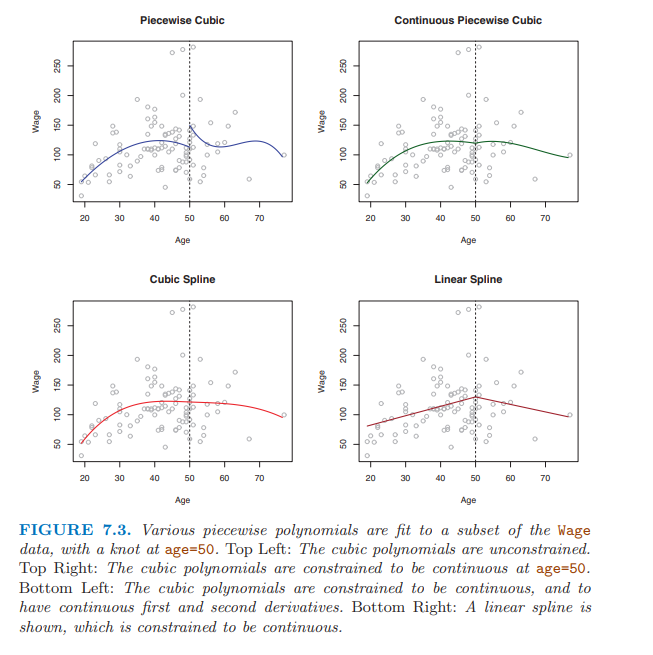
\includegraphics[scale=0.6]{images/B-spline.png}
\end{center}
It  looks wrong because the fitted curve is just too flexible. To remedy this problem, we can fit a piecewise polynomial under the constraint that the fitted curve must be continuous. The top right plot in the Figure shows the resulting fit. This looks better than the top left plot, but the V-shaped join looks unnatural.\\\\
In the lower left plot, we have added two additional constraints: now both
the first and second derivatives of the piecewise polynomials are continuous at $age=50$. In other words, we are requiring that the piecewise polynomial
be not only continuous when $age=50$, but also very \textit{smooth}. So in the top left plot, we are using eight degrees of freedom, but in the bottom left plot we imposed three constraints (continuity, continuity of the first derivative, and continuity of the second derivative) and so are left with five degrees of freedom. The curve in the bottom left plot is called a \textit{cubic spline}. In general, a cubic spline with $K$ knots uses a total of $4 + K$ degrees of freedom.\\\\
The general definition of a degree-$d$ spline is that it is a piecewise degree-$d$ polynomial, with continuity in derivatives up to degree $d - 1$ at each knot. In order to determine the degrees of freedom of a degree-$d$ spline with $K$ knots, we can use the following formula:
\[(d+1)(K+1) - dK\]

\subsection{The Spline Basis Representation}
How can we fit a piecewise degree-$d$ polynomial under the constraint that it (and possibly its first $d - 1$ derivatives) be continuous? It turns out that we can use the basis model \ref{basis} to represent a regression spline. A cubic spline with $K$ knots can be modeled as
\begin{equation}
    y_i = \beta_0 + \beta_1b_1(x_i) + \beta_2b_2(x_i) + ... + \beta_{K+3}b_{K+3}(x_i) + \epsilon_i
    \label{reg-spline}
\end{equation}
for an appropriate choice of basis functions $b_1, b_2,...,b_{K+3}$. The model \ref{reg-spline} can then be fit using least squares.\\\\
The most direct way to represent a cubic spline using \ref{reg-spline} is to start off with a basis for a cubic polynomial, namely, $x, x^2, x^3$, and then add one \textit{truncated power basis} function per knot. A truncated power basis function is defined as 
\begin{equation}
    h(x, \xi) = (x - \xi)^3_+ = 
    \begin{cases}
        (x - \xi)^3 & \text{if } x > \xi\\
        0 & \text{otherwise}
    \end{cases}
\end{equation}
where $\xi$ is the knot. One can show that adding a term of the form $\beta_4h(x, \xi)$ to the model \ref{cubic-pol} for a cubic polynomial will lead to a discontinuity in only the third derivative at $\xi$; the function will remain continuous, with continuous first and second derivatives, at each of the knots.\\\\
In other words, in order to fit a cubic spline to a data set with $K$ knots, we
perform least squares regression with an intercept and $3 + K$ predictors, of the form $X, X^2, X^3, h(X, \xi_1), h(X, \xi_2), ..., h(X, \xi_K)$, where $\xi_1, \xi_2, ..., \xi_K$ are the knots. This amounts to estimating a total of $K + 4$ regression coefficients;  for this reason, fitting a cubic spline with $K$ knots uses $K+4$ degrees of freedom. In general, for a degree-$d$ spline we need $d$ parameters plus one parameter per knot and the intercept.\\\\
Unfortunately, splines can have high variance at the outer range of the predictors, that is, when $X$ takes on either a very small or very large value. A \textit{natural spline} is a regression spline with additional \textit{boundary constraints}: the function is required to be linear at the boundary. This additional constraint means that natural splines are less flexible than regression splines (a natural spline with $K$ knots has $K$ degrees of freedom), and generally produces more stable estimates at the boundaries.

\subsection{Choosing the Number and Locations of the Knots}
When we fit a spline, where should we place the knots? The regression spline is most flexible in regions that contain a lot of knots, because in those regions the polynomial coefficients can change rapidly. Hence, one option is to place more knots in places where we feel the function might vary most rapidly, and to place fewer knots where it seems more stable. While this option can work well, in practice it is common to place knots in a uniform fashion. One way to do this is to specify the desired degrees of freedom, and then have the software automatically place the corresponding number of knots at uniform quantiles of the data.\\\\
How many knots should we use, or equivalently how many degrees of freedom should our spline contain? One option is to try out different numbers of knots and see which produces the best looking curve. A somewhat more objective approach is to use cross-validation.

\subsection{Comparison to Polynomial Regression}
Regression splines often give superior results to polynomial regression. This
is because unlike polynomials, which must use a high degree (exponent in
the highest monomial term, e.g. $X^{15}$) to produce flexible fits, splines introduce flexibility by increasing the number of knots but keeping the degree
fixed. Then, a degree-15 polynomial function will assume very strange shapes more likely to overfit the data. Instead, a regression spline with the same flexibility (in terms of numbers of parameters) can be obtained with a cubic spline with 12 knots, which will produce a smoother fit less sensible to overfitting.

\section{Smoothing Splines}
\subsection{ An Overview of Smoothing Splines}
In the last section we discussed regression splines, which we create by specifying a set of knots, producing a sequence of basis functions, and then using least squares to estimate the spline coefficients. We now introduce a somewhat different approach that also produces a spline.\\\\
In fitting a smooth curve to a set of data, what we really want to do is find some function, say $g(x)$, that fits the observed data well: that is, we want RSS to be small. However, there is a problem with this approach. If we don’t put any constraints on $g(x_i)$, then we can always make RSS zero simply by choosing $g$ such that it interpolates all of the $y_i$, leading to overfitting. What we really want is a function g that makes RSS small, but that is also smooth.\\\\
How might we ensure that $g$ is smooth? There are a number of ways to do this. A natural approach is to find the function $g$ that minimizes
\begin{equation}
    \sum_{i=1}^n (y_i - g(x_i))^2 + \lambda \int g''(t)^2 dt
    \label{smoothing-spline}
\end{equation}
where $\lambda$ is a nonnegative tuning parameter. The function g that minimizes \ref{smoothing-spline} is known as a \textit{smoothing spline}. Equation \ref{smoothing-spline}  takes the “Loss+Penalty” formulation that we encounter in the context of ridge regression and the lasso. The first term is a \textit{loss function} that encourages $g$ to fit the data well, while the second term is a \textit{penalty term} hat penalizes the variability in $g$. The notation $g''(t)$ indicates the second derivative of the function $g$. The first derivative $g'(t)$
measures the slope of a function at $t$, and the second derivative corresponds to the amount by which the slope is changing. Hence, the second derivative is large in absolute value if $g(t)$ is very wiggly near $t$, and it is close to zero otherwise. The integral simply measures the total change in the function $g'(t)$, over its entire range. If $g$ is very smooth, then $g'(t)$ will be close to constant and $\int g''(t)^2 dt$ will take on a small value. Conversely, if $g$ is jumpy and variable, $\int g''(t)^2 dt$ will take on large values.\\\\
The larger the value of $\lambda$, the smoother $g$ will be. When $\lambda \rightarrow \infty$, $g$ will be perfectly smooth—it will just be a straight line that passes as closely as possible to the training points. In fact, in this case, $g$ will be the linear least squares line.\\\\
The function $g(x)$ that minimizes \ref{smoothing-spline}  can be shown to have some special properties: it is a piecewise cubic polynomial with knots at the unique
values of $x_1,...,x_n$, and continuous first and second derivatives at each knot. Furthermore, it is linear in the region outside of the extreme knots. In other words, the function $g(x)$ that minimizes \ref{smoothing-spline} is a natural cubic
spline with knots at $x_1,...,x_n$. However, it is not the same natural cubic
spline that one would get if one applied the basis function approach described previously with knots at $x_1,...,x_n$. Rather, it is a \textit{shrunken} version of such a natural cubic spline, where the value of the tuning parameter $\lambda$ controls the level of shrinkage.

\subsection{Choosing the Smoothing Parameter $\lambda$}
We have seen that a smoothing spline is simply a natural cubic spline with knots at every unique value of $x_i$. It might seem that a smoothing spline will have far too many degrees of freedom, since a knot at each data point allows a great deal of flexibility. But the tuning parameter $\lambda$ controls the roughness of the smoothing spline, and hence the \textit{effective degrees of freedom}.\\\\
In the context of smoothing splines, why do we discuss effective degrees of freedom instead of degrees of freedom? Usually degrees of freedom refer to the number of free parameters, such as the number of coefficients fit in a polynomial or cubic spline. Although a smoothing spline has $n$ parameters and hence $n$ nominal degrees of freedom, these $n$ parameters are heavily constrained or shrunk down. Hence $df_\lambda$ is a measure of the flexibility of the smoothing spline, the higher it is, the more flexible the smoothing spline.\\\\
In fitting a smoothing spline, we do not need to select the number or location of the knots. Instead, we have another problem: we need to choose the value of $\lambda$. It should come as no surprise that one possible solution to this problem
is cross-validation. It turns out that the \textit{leaveone-out} cross-validation error (LOOCV) can be computed very efficiently for smoothing splines.

\section{Generalized Additive Models}
In the previous sections we present a number of approaches for flexibly predicting a response $Y$ on the basis of a single predictor $X$. Here we explore the problem of flexibly predicting $Y$ on the basis of several predictors, $X_1,...,X_p$.\\\\
Generalized additive models (GAMs) provide a general framework for extending a standard linear model by allowing non-linear functions of each of the variables, while maintaining \textit{additivity}.

\subsection{GAMs for Regression Problems}
A natural way to extend the multiple linear regression model in order to allow for non-linear relationships between each feature and the response is to replace each linear component $\beta_jx_{ij}$ with a (smooth) nonlinear function $f_j(x_{ij})$. We would then write the model as
\begin{equation}
    y_i = \beta_0 + \sum_{j=1}^p f_j(x_{ij}) + \epsilon_i
\end{equation}
In the previous sections, we discussed many methods for fitting functions to a single variable. The beauty of GAMs is that we can use these methods as building blocks for fitting an additive model.\\\\
Fitting a GAM with a smoothing spline is not quite as simple as fitting a GAM with a natural spline, since in the case of smoothing splines, least squares cannot be used. However, standard software can be used to fit GAMs using smoothing splines, via an approach known as backfitting.

\subsection{Pros and Cons of GAMs}
Let us summarize the advantages and limitations of a GAM.\\\\
\textbf{Pros:}
\begin{itemize}
    \item GAMs allow us to fit a non-linear $f_j$ to each $X_j$ , so that we can automatically model non-linear relationships that standard linear regression will miss.

    \item The non-linear fits can potentially make more accurate predictions for the response $Y$.

    
    \item Because the model is additive, we can still examine the effect of each $X_j$ on $Y$ individually while holding all of the other variables fixed.

    \item The smoothness of the function $f_j$ for the variable $X_j$ can be summarized via degrees of freedom.
\end{itemize}
\textbf{Cons:}
\begin{itemize}
    \item The main limitation of GAMs is that the model is restricted to be additive. With many variables, important interactions can be missed. However, as with linear regression, we can manually add interaction terms to the GAM model by including additional predictors of the form $X_j \times X_k$.
\end{itemize}

